\section{Durchführung des Experiments}
Nachdem der Testaufbau besprochen wurde, gilt es nun in die Rolle des Angreifers
zu schlüpfen und mögliche Angriffe zu diskutieren und auszuführen. Außerdem soll
besprochen werden, wie die Angriffe hätten verhindert werden können, sodass die
Arbeit von~\cite{paper} Anwendung findet. Wie in
Abbildung~\ref{fig:testing-setup} dargestellt, werden die Komponenten zunächst
aufgebaut. Folgende Netzwerkteilnehmer werden konfiguriert:

\begin{itemize}
  \item \textbf{Alice} erhält die IP-Adresse 192.168.2.115 und stellt einen
    MQTT-Client dar. Es werden bestimmte Topics abonniert, sodass dieses Gerät
    benachrichtigt wird, falls sich bestimmte Werte im System ändern.
  \item \textbf{Bob} erhält die IP-Adresse 192.168.2.171 und stellt den
    MQTT-Broker dar. Dieser empfängt Daten von Sensoren und speichert diese
    unter einem bestimmten Topic ab. Abonnenten des Topics werden dann von ihm
    benachrichtigt. Als Anwendung wird \textit{Aedes} verwendet.
  \item Der \textbf{Sicherheitskamera} (Security Camera) wird die IP-Adresse
    192.168.2.178 zugewiesen und dient in dem Aufbau als Sensor. Es werden
    periodisch Bildaufnahmen erzeugt und an Bob gesendet.
  \item \textbf{Eve} stellt den Angreifer dar und erhält die IP-Adresse
    192.168.2.168.
  \item Der \textbf{Router} stellt mit der IP-Adresse 192.168.2.1 das
    Standard-Gateway des Netzwerks dar.
\end{itemize}

\subsection{Eavesdropping}
Ein entscheidender Grund, warum HTTPS als Ergänzung zu HTTP entwickelt wurde,
ist das Senden und Empfangen von sensiblen Informationen wie Passwörter und
anderen benutzerspezifischen Eigenschaften. Dies ist auch bei MQTT bzw. MQTTS
der Fall. Deshalb wird in diesem Abschnitt untersucht, wie sicher das Framework
\textit{pi-aREST} diesbezüglich ist. Als erster Punkt kann genannt werden, dass
es nicht möglich ist, den Kommunikationsport einzustellen. Dieser ist fest in
das Framework eingearbeitet und lautet 1883, was auf einen unverschlüsselten
Kanal hinweist. Da die Ports jedoch vom Serveradministrator individuell
verwendet werden können, muss nun untersucht werden, ob die Kommunikation
tatsächlich unverschlüsselt verläuft. Hierfür wird auf \textit{Eve} das
Netzwerkanalyse-Tool \textit{Wireshark} installiert und ausgeführt. Zudem werden
die Dienste von der Sicherheitskamera und Bob gestartet, sodass diese
miteinander kommunizieren und Daten kontinuierlich ausgetauscht werden. Werden
Pakete von einem Netzwerkteilnehmer zu einem anderen gesendet, sind diese an
jedem Knotenpunkt im Netzwerk abgreifbar. Jeder Knotenpunkt entscheidet dann
anhand der Paket-Header, ob das jeweilige Paket für ihn bestimmt ist. Dadurch,
dass in der Tat keine Verschlüsselung der Daten erfolgt, können mithilfe von
\textit{Wireshark} Bildaufnahmen ausgespäht werden, wie
Abbildung~\ref{fig:wireshark} zeigt. Gerade bei Kameras, die im Grunde nie für
jedermann zugänglich sein sollen, ist dies eine große Sicherheitslücke. Diese
könnte beispielsweise durch ein geeignetes Verschlüsselungsverfahren geschlossen
werden, sodass nur Parteien mit den jeweiligen geheimen Schlüsseln Zugriff zu
den Daten erlangen können. Dieses Experiment zeigt, dass durch simples Zuhören
sensible Daten ausgespäht werden können, ohne in den Informationsfluss
einzugreifen oder zu beeinflussen. Voraussetzung ist natürlich, dass sich der
Angreifer im selben Netzwerk befindet.

\begin{figure}
  \centerline{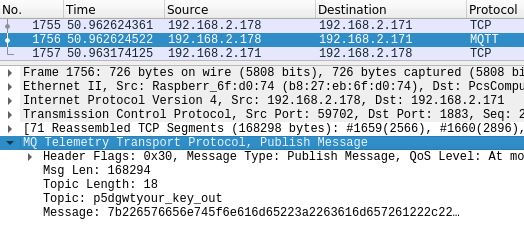
\includegraphics[width=\columnwidth]{images/wireshark}}
  \caption{Ausgespähte Pakete des unsicheren MQTT-Protokolls mit Wireshark}
  \label{fig:wireshark}
\end{figure}

\subsection{Man-in-the-Middle-Angriff}
Bei einem Blackhole-Angriff handelt es sich um einen Denial-of-Service-Angriff
(DoS), bei dem die Verfügbarkeit der Daten angegriffen wird. Dabei wird der
Informationsfluss zwischen zwei Knotenpunkten über eine dritte Instanz
umgeleitet. Anschließend werden bestimmte Informationspakete verworfen, sodass
diese dem eigentlichen Ziel nicht mehr zur Verfügung stellen~\cite{aad2004}. Als
würden die Informationen in ein schwarzes Loch fallen.

Auch dies soll in diesem Experiment durchgeführt werden. Hierfür werden die
Dienste von Bob und der Sicherheitskamera gestartet, sodass ein
Informationsfluss stattfindet. Es werden also wieder kontinuierlich Bilder von
der Kamera aufgenommen und an den Broker gesendet. Das Ziel in diesem Versuch
ist es, die Verbindung zu unterbrechen bzw. Pakete verschwinden zu lassen, ohne
einen einzelnen Knotenpunkt auszuschalten, wie es bei einem DDoS-Angriff der
Fall ist. Die erste Hürde ist also, sich als Angreifer zwischen die beiden
Kommunikationspartner zu schalten, ohne dass diese es bemerken. Ein solcher
Angreifer wird traditionell als \textit{Man in the Middle} (MitM) bezeichnet. Es
stellt sich nun also die Frage, wie man den Informationsfluss über eine dritte
Instanz leiten kann. Die einfachste Methode ist das ARP-Spoofing. Hierbei werden
den beiden Teilnehmern vorgetäuscht, man selbst sei der richtige
Gesprächspartner.

Das \textit{Address Resolution Protocol} (ARP) ist ein häufig eingesetztes
Protokoll, welches Adressen des \textit{Internet Protocols} (IP) auf Adressen
des \textit{Link-Layers} (MAC-Adressen) abbildet. Teilnehmer des Netzwerks,
welches ARP verwendet, nehmen alle ARP-Pakete an, egal wer diese sendet. Dies
hat vor allem Performance-Gründe, bildet jedoch eine wichtige Schwachstelle für
einen MitM-Angriff im lokalen Netzwerk.

Eve hat nun also die Aufgabe, sich bei Bob als die Sicherheitskamera und bei der
Sicherheitskamera sich als Bob auszugeben. Hierbei wird eine Schwachstelle des
ARP-Protokolls ausgenutzt. ARP implementiert nämlich keine Authentifizierung der
Knotenpunkte, die das Protokoll verwenden. Als Angreifer sendet Eve also
ARP-Pakete, mit denen sie Bob weiß macht, sie sei die Sicherheitskamera. Bob
merkt sich dies und speichert sich den Eintrag in seine persönliche ARP-Tabelle.
Anschließend gibt sich Eve als Bob bei der Sicherheitskamera aus und sendet
entsprechende ARP-Pakete zu ihr. Auch diese merkt sich dies in ihrer eigenen
Tabelle. Hiermit verläuft der Informationsfluss zwischen der Sicherheitskamera
und Bob über Eve. Damit Pakete nun tatsächlich weitergeleitet werden, müsste
dies erst konfiguriert werden. Wird dies nicht getan, werden alle Pakete
einfach bis zu Eve gelangen und dann verworfen werden, also genau das, was das
Ziel dieses Versuchs ist. Die Pakete werden somit verschluckt und tauchen nicht
bei dem eigentlichen Ziel auf. Auf das Experiment bezogen bedeutet dies, dass
die aufgenommenen Bilder von der Sicherheitskamera nicht zu dem Broker gelangen
und eine Aktualisierung des entsprechenden Topics ausfällt. Die Verfügbarkeit
wurde damit als grundlegende Sicherheitsanforderung verletzt.

Des Weiteren können nun mächtigere Angriffe durchgeführt werden, wie
beispielsweise das Manipulieren der Bilddaten. Bei einem Einbruch könnte der
Angreifer die Bilder z.B. so verändern, dass dieser nicht auf den Aufnahmen zu
sehen ist. Da das Framework, mit dem die Anwendung entwickelt wurde, lediglich
das MQTT- und nicht das sicherere MQTTS-Protokoll verwendet, kann die Integrität
der Daten nicht gewährleistet werden.
